\documentclass[12pt]{article}
\usepackage{geometry}                % See geometry.pdf to learn the layout options. There are lots.
\geometry{letterpaper}                   % ... or a4paper or a5paper or ... 
%\geometry{landscape}                % Activate for for rotated page geometry
\usepackage[parfill]{parskip}    % Activate to begin paragraphs with an empty line rather than an indent
\usepackage{daves,fancyhdr,natbib,graphicx,dcolumn,amsmath,lastpage,url}
\usepackage{amsmath,amssymb,epstopdf,longtable}
\usepackage{paralist}  % need to modify standard enumerate blocks
\usepackage[final]{pdfpages}
\DeclareGraphicsRule{.tif}{png}{.png}{`convert #1 `dirname #1`/`basename #1 .tif`.png}
\pagestyle{fancy}
\lhead{CE 3354 -- Engineering Hydrology}
\rhead{FALL 2025}
\lfoot{ES2}
\cfoot{}
\rfoot{Page \thepage\ of \pageref{LastPage}}
\renewcommand\headrulewidth{0pt}



\begin{document}
\begin{center}
{\textbf{{ CE 3354 Engineering Hydrology} \\ {Exercise Set 1}}}
\end{center}

\section*{\small{Exercises}}
\begin{enumerate}
\item A farm has a reservoir with vertical sides and surface area of 2.5 acres. Following the reservoir has accumulated 9.84 feet of water.  During the dry season the reservoir loses 2.5 inches of water per week to evaporation.  The average irrigation demand during the dry season is 0.23 acre-ft per day.

Determine:
    \begin{enumerate}[a)]
        \item How many weeks can the farm irrigate water from the reservoir supply? 
    \end{enumerate}

\clearpage
%%%%%%%%%%%%%%%%%%%%%%%%%%%%%%%%%%%%%%%%%%%%%%%%%%%%%%%%%%%%

\item The mean annual precipitation for a certain 132 square-mile watershed is 25 inches. Assume that 20 percent of the annual precipitation reaches the watershed outlet as streamflow.

Determine:
    \begin{enumerate}[a)]
        \item The mean streamflow rate in acre-feet per year. 
        \item The mean streamflow rate in cubic-feet per second.
        \item The mean streamflow rate in cubic-meters per second.
    \end{enumerate}

\clearpage
%%%%%%%%%%%%%%%%%%%%%%%%%%%%%%%%%%%%%%%%%%%%%%%%%%%%%%%
\item The mean annual rainfall depth over a 280 km$^2$ watershed is 725 mm.

Determine:
    \begin{enumerate}[a)]
        \item The mean annual volume of rain falling on the watershed in cubic meters. 
        \item The mean annual volume of rain falling on the watershed in cubic feet.
        \item The mean annual volume of rain falling on the watershed in gallons.
        \item The mean annual volume of rain falling on the watershed in acre-feet.
    \end{enumerate}

\clearpage
%%%%%%%%%%%%%%%%%%%%%%%%%%%%%%%%%%%%%%%%%%%%%%%%%%%%%%%%%
\item Figure \ref{fig:farmland} is a schematic of a 600-hectare farm; the land receives annual rainfall of 2500 mm.  There is a river flowing through the farm land with inflow rate of 5 m$^3$/s and outflow rate of 4m$^3$/s.  The annual water storage in the farm land increases by 2.5$\times$10$^6$m$^3$.  Using the water budget concept, estimate the annual evaporation amount in millimeters.\footnote{1 hectare = 10,000 m$^2$}

\begin{figure}[h!] %  figure placement: here, top, bottom, or page
   \centering
   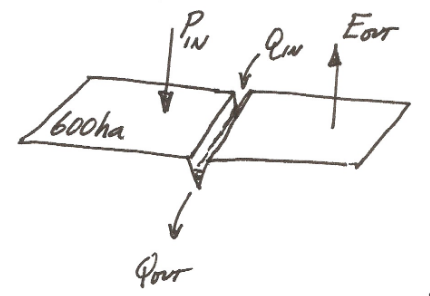
\includegraphics[width=4in]{farmland.png} 
   \caption{Schematic of Farmland}
   \label{fig:farmland}
\end{figure}
\clearpage
%%%%%%%%%%%%%%%%%%%%%%%%%%%%%%%%%%%%%%%%%%%%%%%%%%%%%%%%%
\item A reservoir has a surface area of 690 acres.  Figure \ref{fig:reservoir} shows the monthly inflow of surface water, outflows as releases from the reservoir via the spillway, direct precipitation into the reservoir, and evaporation from the reservoir.  The reservoir water surface elevation was 701.0 feet on January 1.  Determine the reservoir water surface elevation at the end of each month (i.e. complete the table)

\begin{figure}[h!] %  figure placement: here, top, bottom, or page
   \centering
   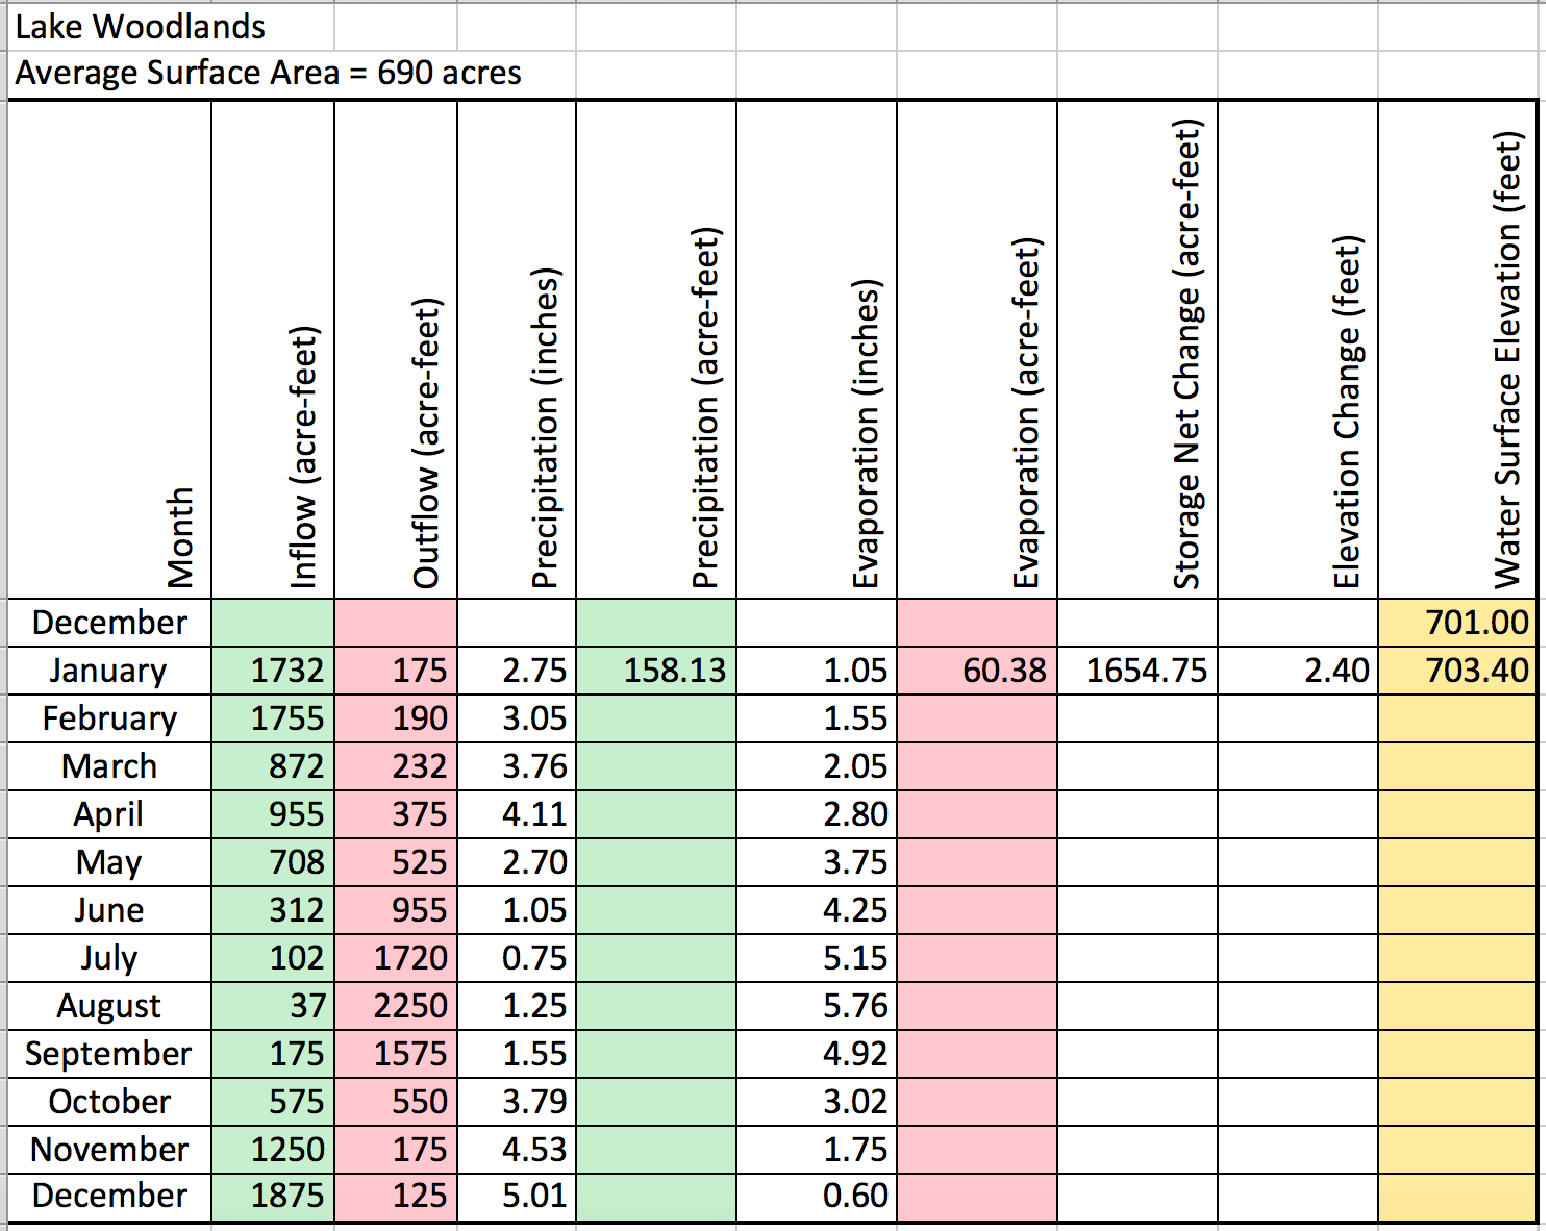
\includegraphics[width=6in]{Reservior.pdf} 
   \caption{Tabular Water Budget Values}
   \label{fig:reservoir}
\end{figure}


    
\end{enumerate}


\end{document}  

%%%%%%%%%%%%%%%%%%%%%%%%%%%%%%%%%%%%%%%%%%%%%%%%%%%%%%%
\item The map in Figure \ref{fig:polygonmap} shows the location of 6 rain gages and a watershed boundary. The rainfall depths for a certain storm are shown by each gage. An isohyetal map is displayed on the figure as is a linear distance scale.

\begin{figure}[h!] %  figure placement: here, top, bottom, or page
   \centering
   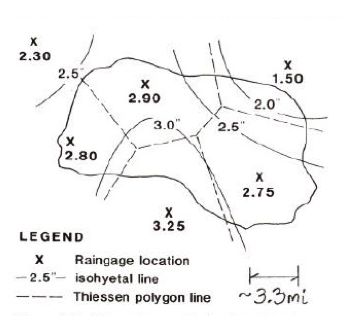
\includegraphics[height=4in]{polygonmap.png} 
   \caption{Raingages}
   \label{fig:polygonmap}
\end{figure}

Determine:
    \begin{enumerate}[a)]
        \item The Theissen polygon boundaries – verify if the gage in the upper left corner is included in the polygon boundaries in the picture (i.e determine your own boundaries for the gages, do they agree with the drawing?). 
        \item The polygon areas and compute the Theissen weights.
        \item The average weighted precipitation over the watershed (using the Theissen weights).
        \item The average weighted precipitation (using the Isoheyets).
    \end{enumerate}
\clearpage
~\newline
\clearpage
%%%%%%%%%%%%%%%%%%%%%%%%%%%%%%%%%%%%%%%%%%%%%%%%%%%%%%%
\item The map in Figure \ref{fig:gagemap} shows the location of 8 rain gages and the watershed boundary. The rainfall depths for a certain storm are in Table \ref{tab:gagemap}. Use the Thiessen polygon method to determine the mean rainfall depth over the watershed for this storm event.

\begin{figure}[h!] %  figure placement: here, top, bottom, or page
   \centering
   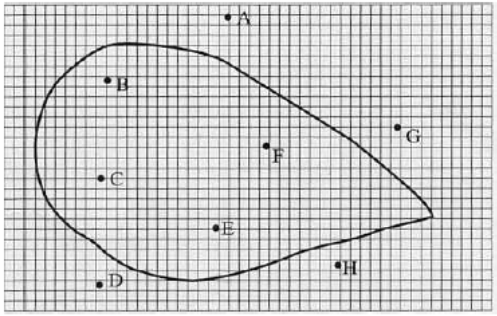
\includegraphics[height=3in]{gagemap.png} 
   \caption{Nowhere Watershed Active Raingages}
   \label{fig:gagemap}
\end{figure}

\begin{table}[h!]
\centering
\caption{Nowhere Watershed Precipitation}
\begin{tabular}{p{2.0in}p{2.0in}} % Column formatting, @{} suppresses leading/trailing space
~&~\\
Gage & Cumulative Depth (millimeters)\\
\hline
\hline
A & 25.00 \\
B & 18.00 \\
C & 92.00 \\
D & 95.00 \\
E & 192.0 \\
F & 175.0 \\
G & 152.0 \\
H & 168.0 \\

\hline
\end{tabular}
\label{tab:gagemap}
\end{table}

Determine:
    \begin{enumerate}[a)]
        \item The mean rainfall depth over the watershed for this storm event using the arithmetic mean. 
        \item The mean rainfall depth over the watershed for this storm event using the Thiessen polygon method. 
    \end{enumerate}

\clearpage
%%%%%%%%%%%%%%%%%%%%%%%%%%%%%%%%%%%%%%%
~\newline